\clearpage
\section{Non-Functional Requirements}

\subsubsection{Category: User Interface}

\textbf{ID: 1 Consistent Look}
\begin{enumerate}
    \item Description: The user interface must have a consistent blue look  across all pages and maintaining the same color schemes.
    \item Affects: Players and Admins interacting with the platform.
\end{enumerate}

\subsubsection{Category: Security}

\textbf{ID: 2 Secure Authentication}
\begin{enumerate}
    \item Description: The platform must implement secure login mechanisms, including password protection.
    \item Affects: Players and Admins accessing their accounts.
\end{enumerate}

\textbf{ID: 3 Data Protection}
\begin{enumerate}
    \item Description: User data like personal details and game statistics must be encrypted.
    \item Affects: All users
\end{enumerate}

\subsubsection{Category: Performance}

\textbf{ID: 4 Scalability}
\begin{enumerate}
    \item Description: The game should be able to handle multiple players playing.
    \item Affects: All users during peak usage periods.
\end{enumerate}

\subsubsection{Category: Usability}

\textbf{ID: 5 Tutorial Support}
\begin{enumerate}
    \item Description: The game must include a tutorial for players to learn the rules and gameplay mechanics of Go Fish.
    \item Affects: All users
\end{enumerate}

\textbf{ID: 6 Shop}
\begin{enumerate}
    \item Description: The game must include a shop for player to use their earned currency.
    \item Affects: All users
\end{enumerate}

\subsubsection{UI Description}

The following figures showcase the user interface screenshots for our application. Each screenshot highlights a key feature or design aspect. The game begins with a login screen where users can either log in, create an account, or join as a guest, allowing flexibility for both returning and new players. Once logged in, users are presented with a main menu that serves as a hub for navigating the platform. From here, they can access key features like creating or joining game lobbies, visiting the shop to purchase customizations, messaging the admin or starting a tutorial to learn the gameplay. Players choosing to join as guests can also select an avatar for personalization before entering the main menu. To start a game, users can create a public or private lobby, specifying the game mode and player limit. Alternatively, they can join an existing lobby using a code or search for open lobbies. Once in the lobby, players are matched with others, and the game begins. The in game interface provides a clear view of the player's cards, turn order, and actions, such as selecting a player and asking for a card. The game flow ensures a smooth and engaging experience.

\begin{figure}[h!]
\centering
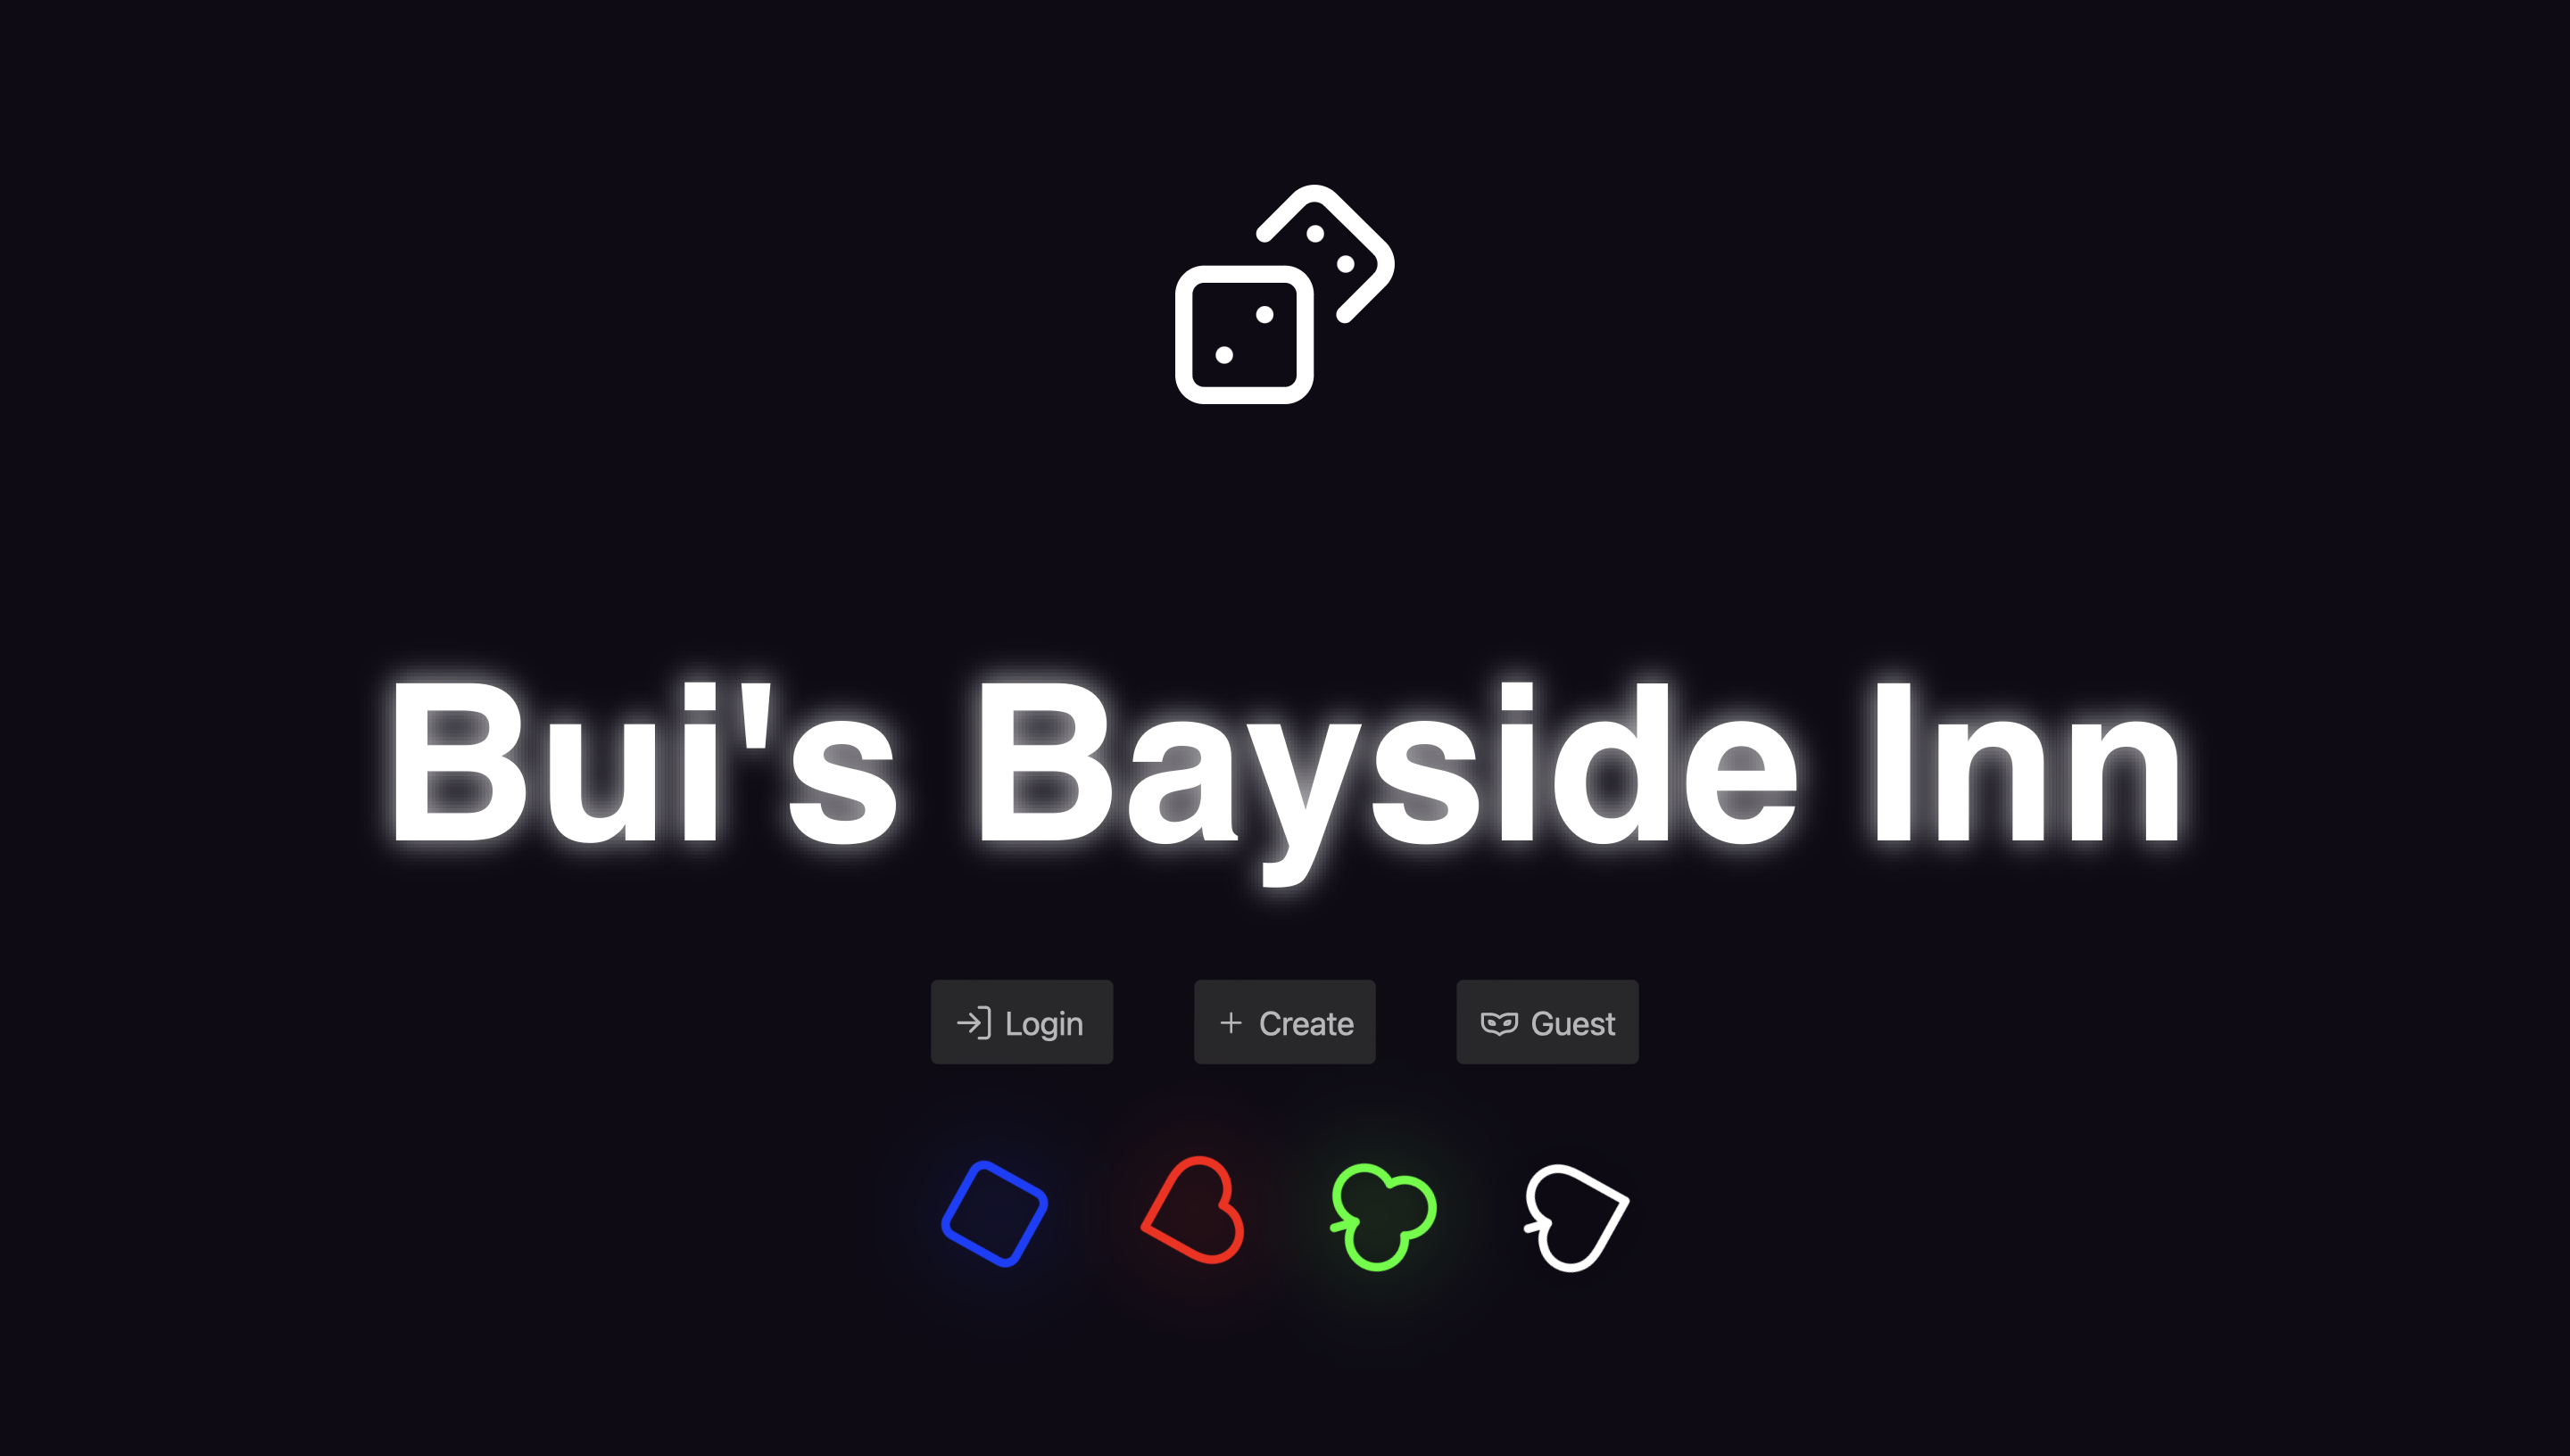
\includegraphics[width=1\linewidth]{UI Screenshot 1.png}
\label{fig:ui1}
\end{figure}

\begin{figure}[h!]
\centering
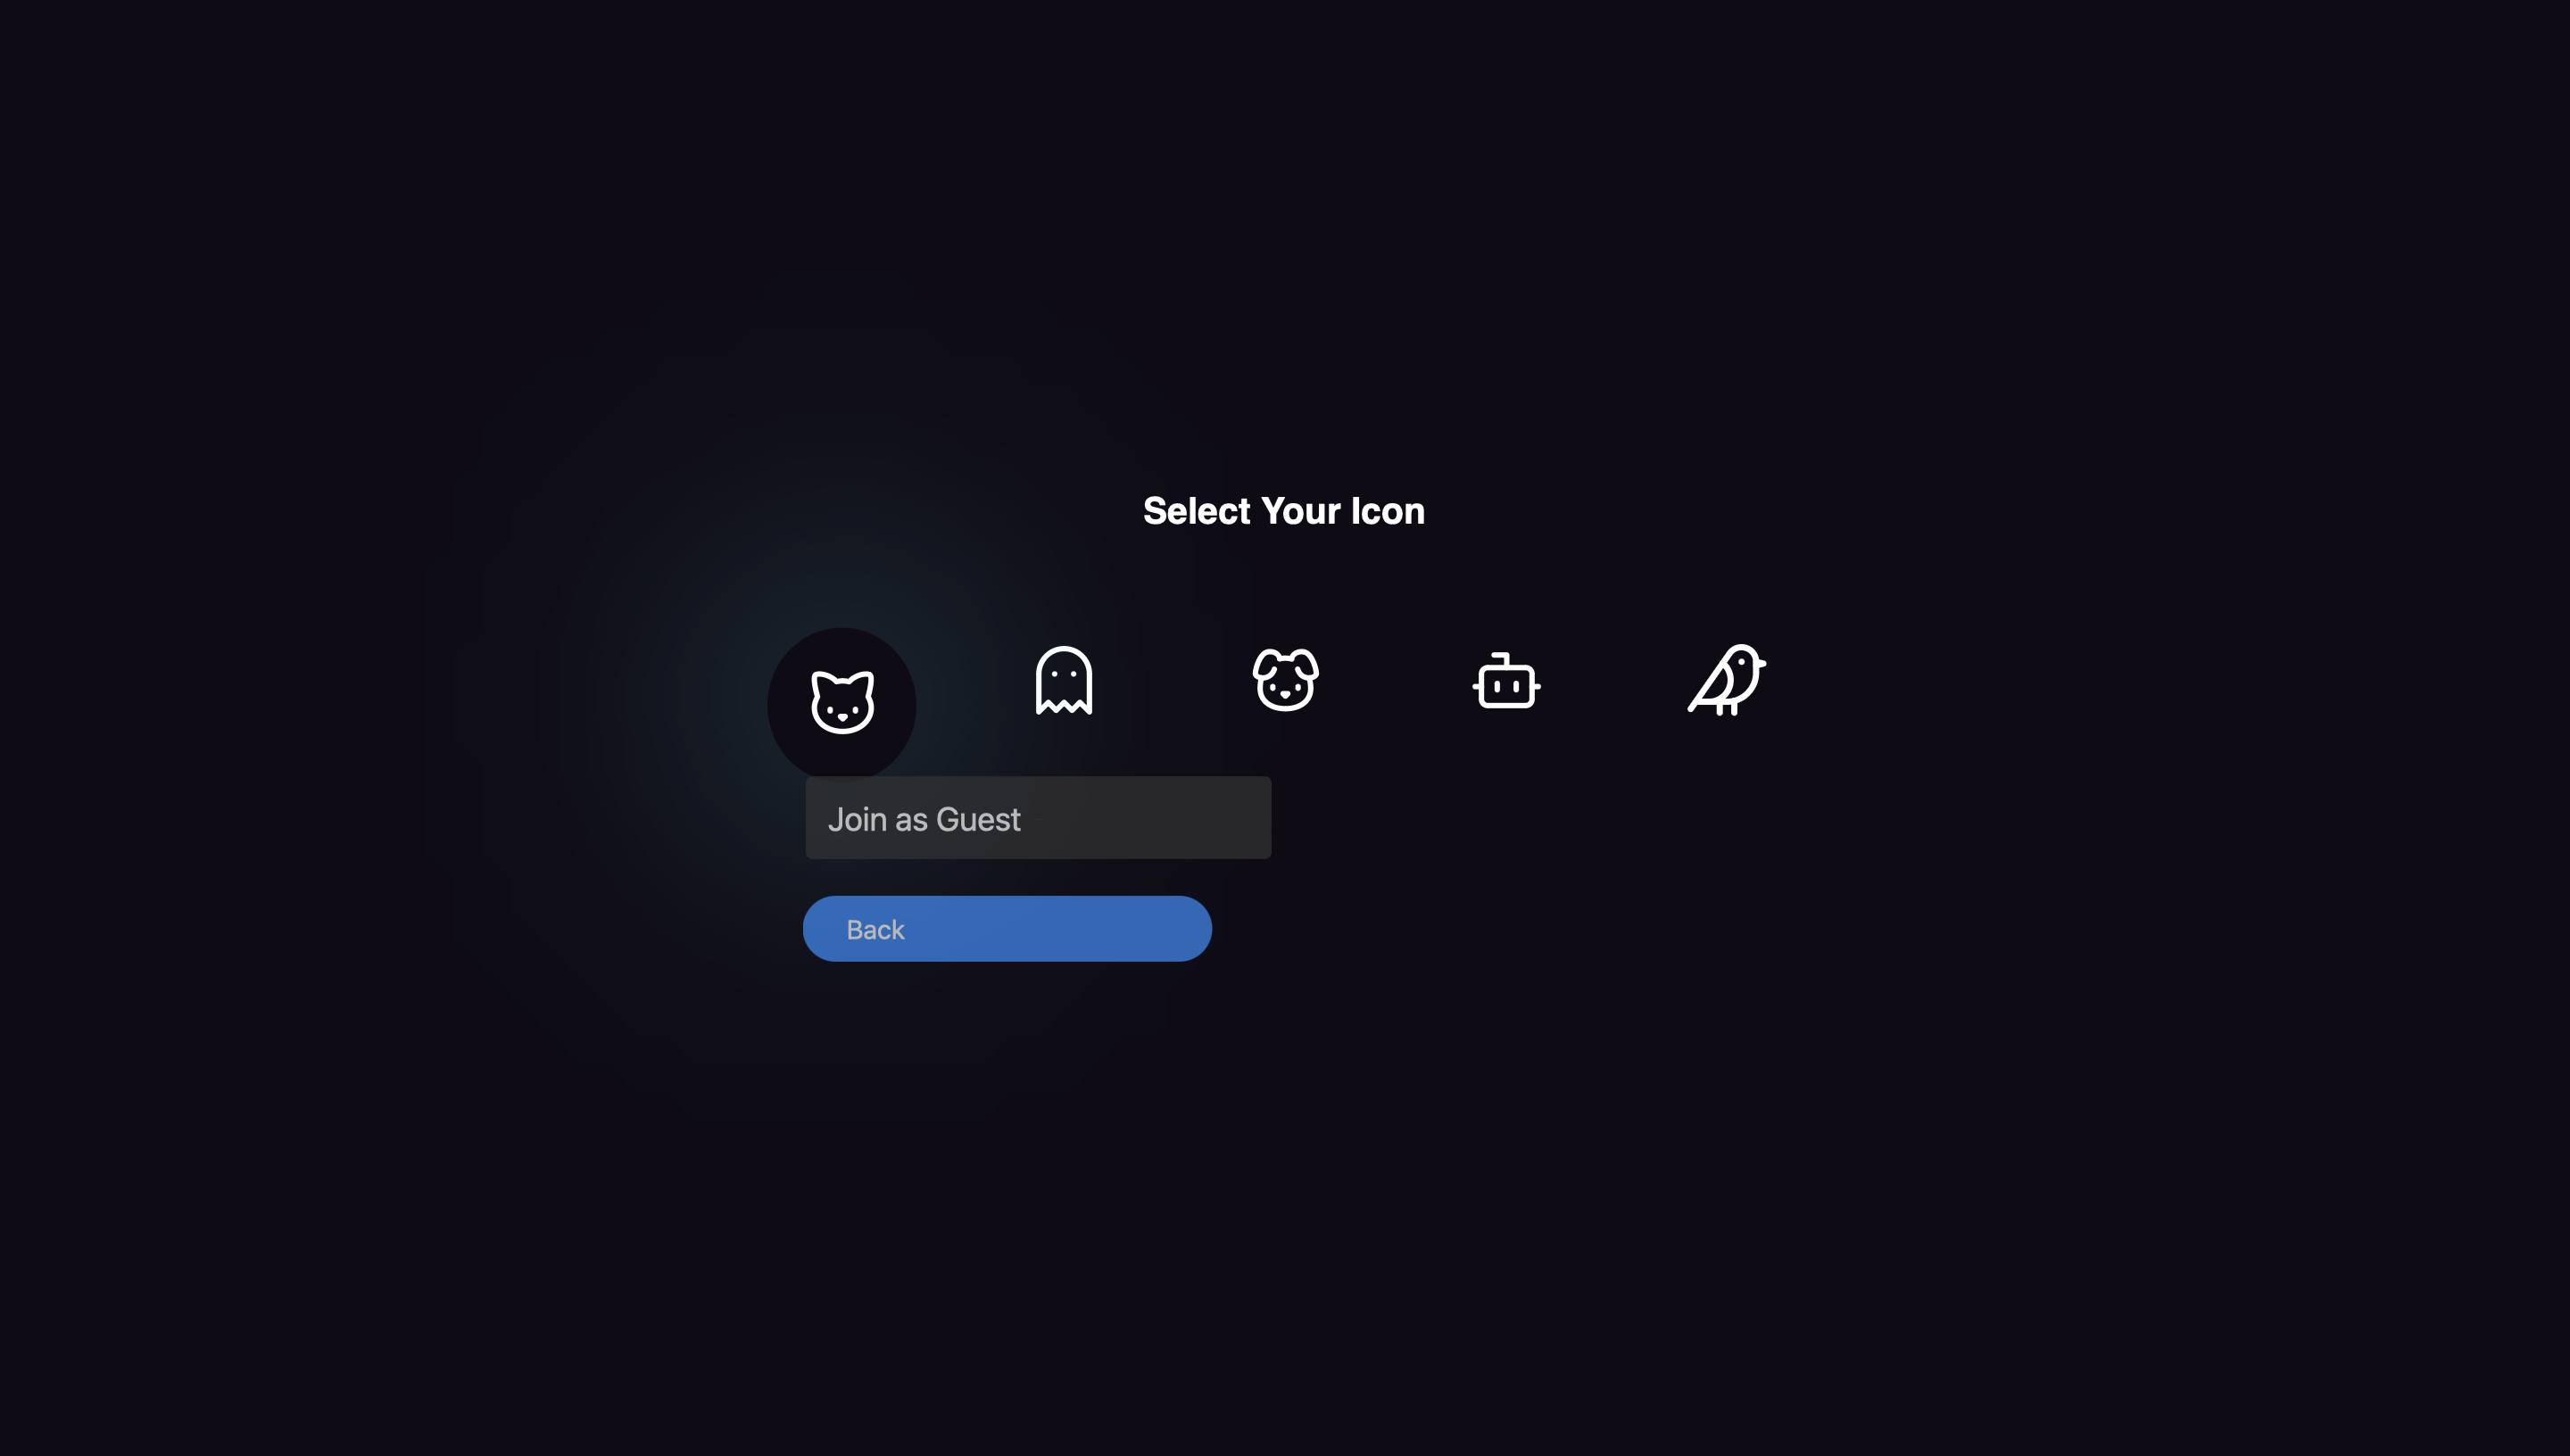
\includegraphics[width=1\linewidth]{UI Screenshot 2.png}
\label{fig:ui2}
\end{figure}

\begin{figure}[h!]
\centering
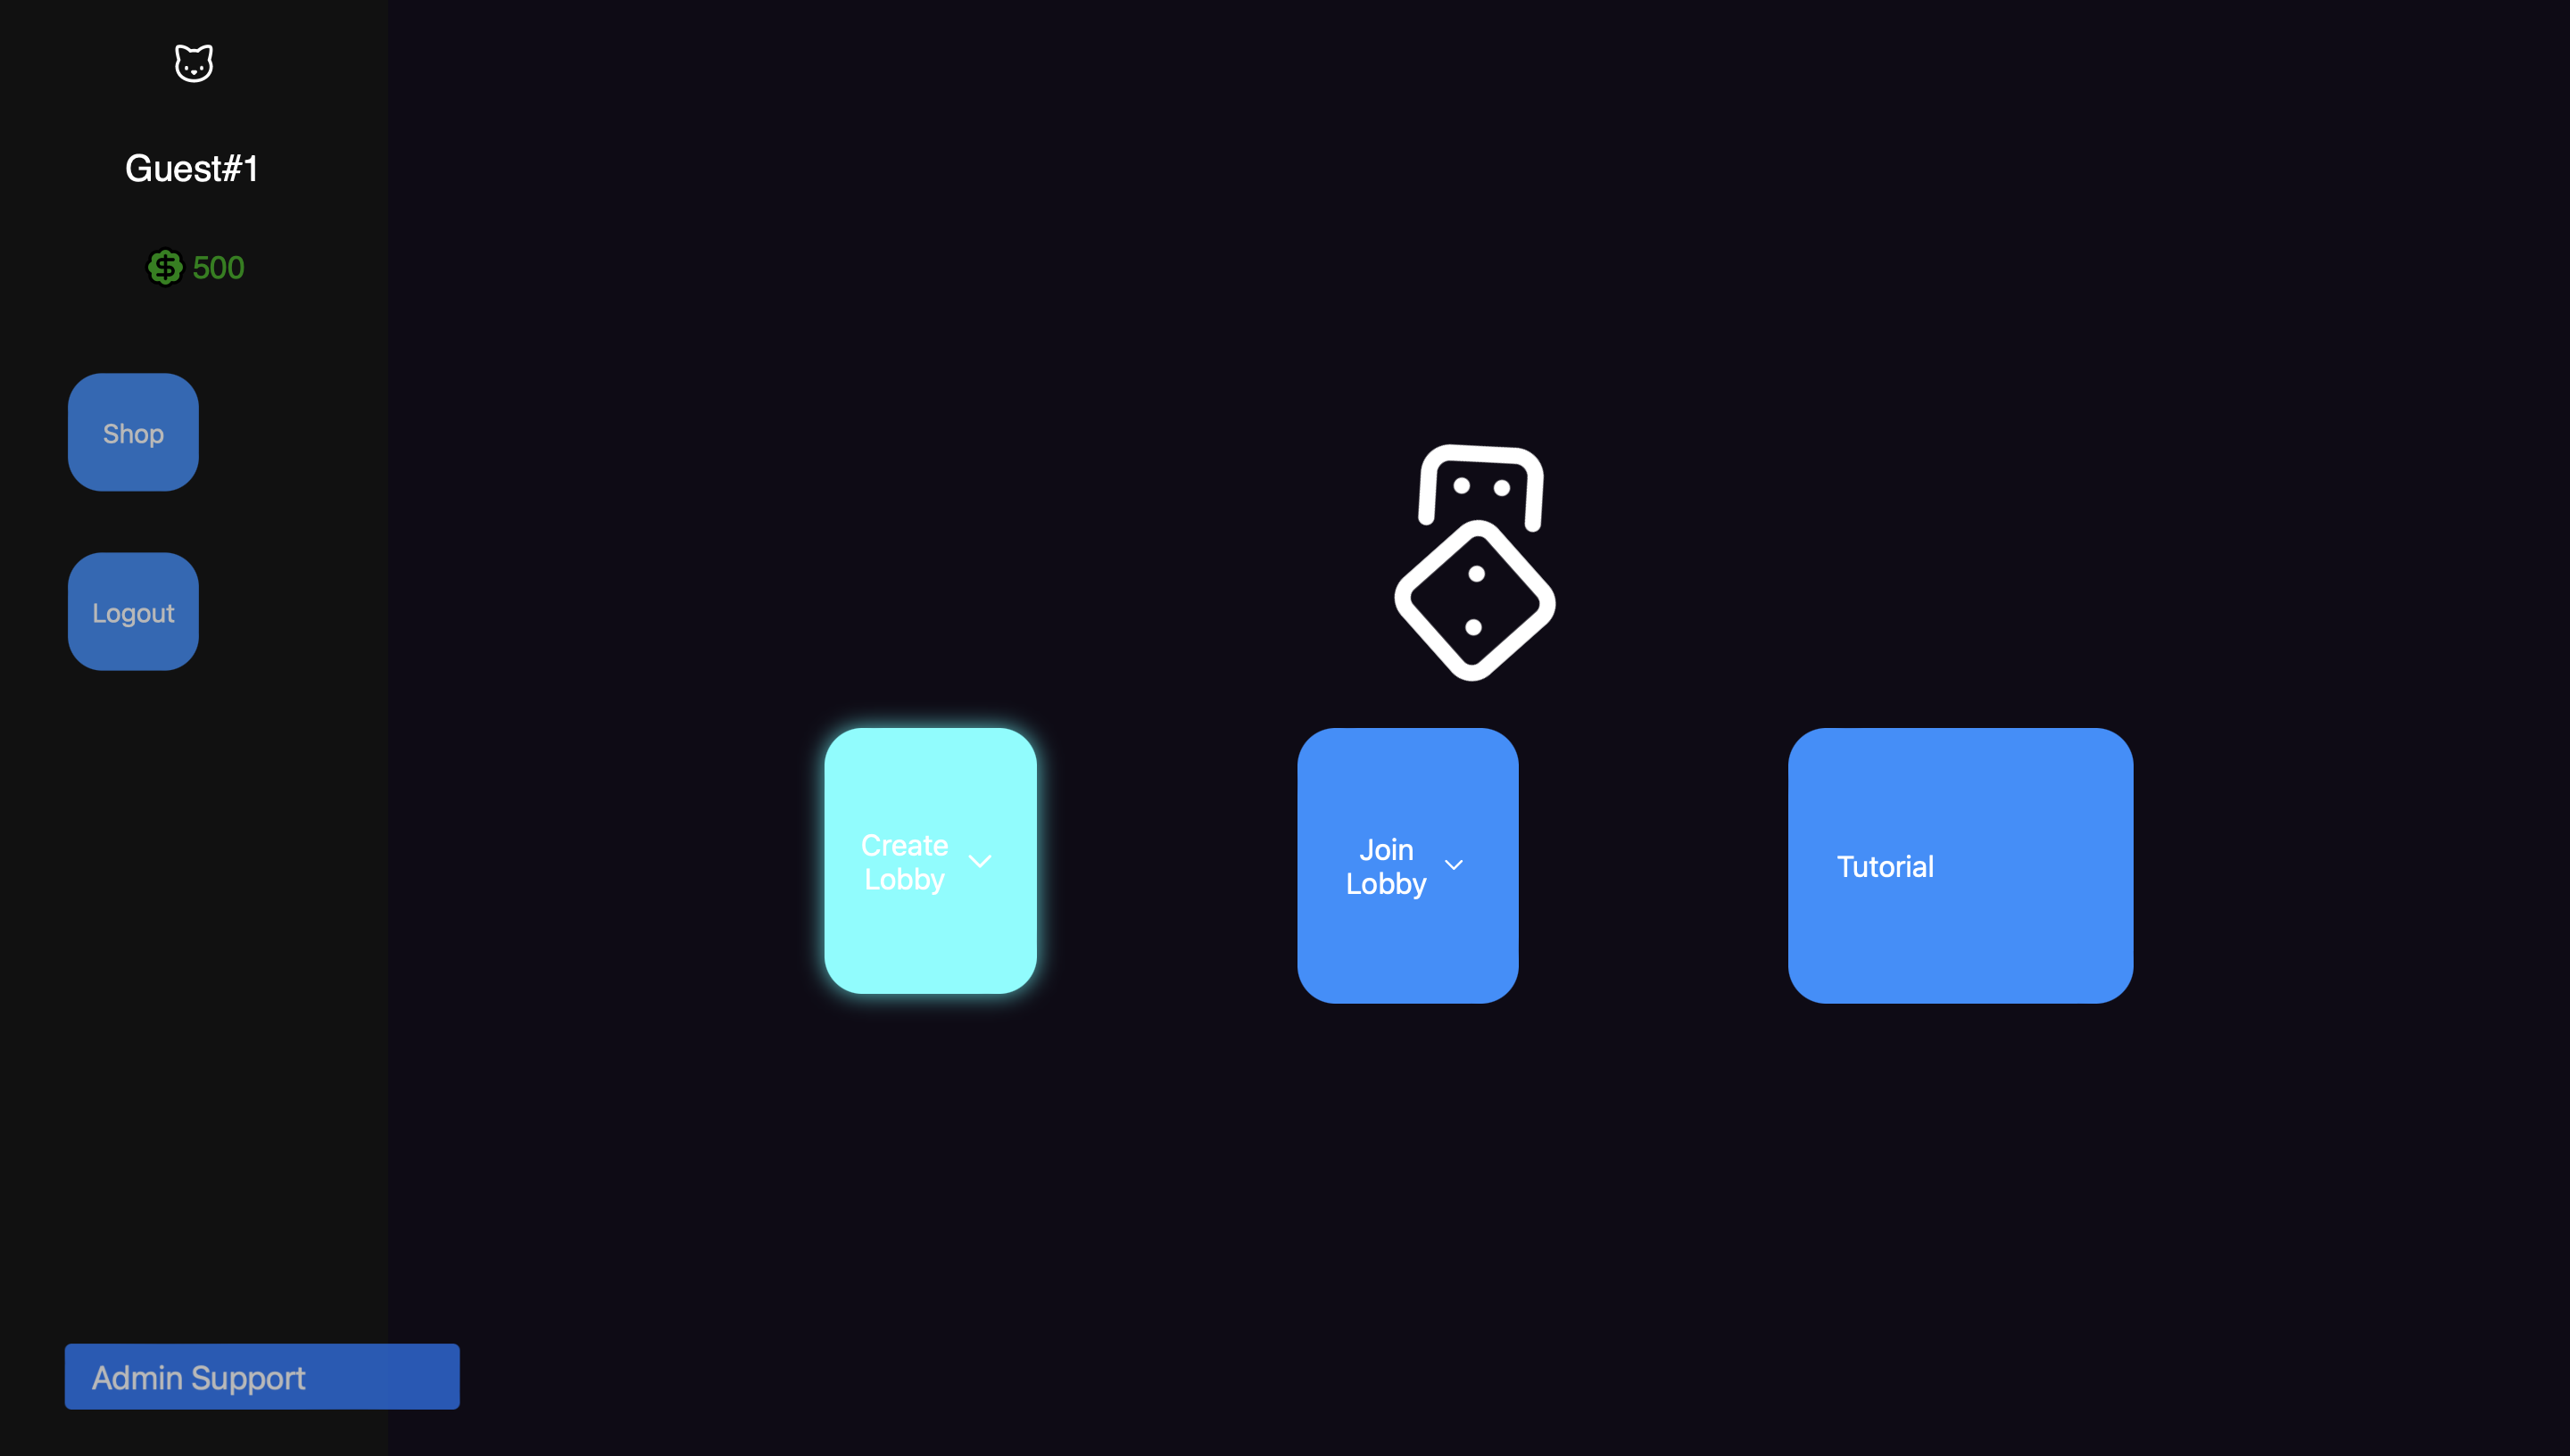
\includegraphics[width=1\linewidth]{UI Screenshot 3.png}
\label{fig:ui3}
\end{figure}

\begin{figure}[h!]
\centering
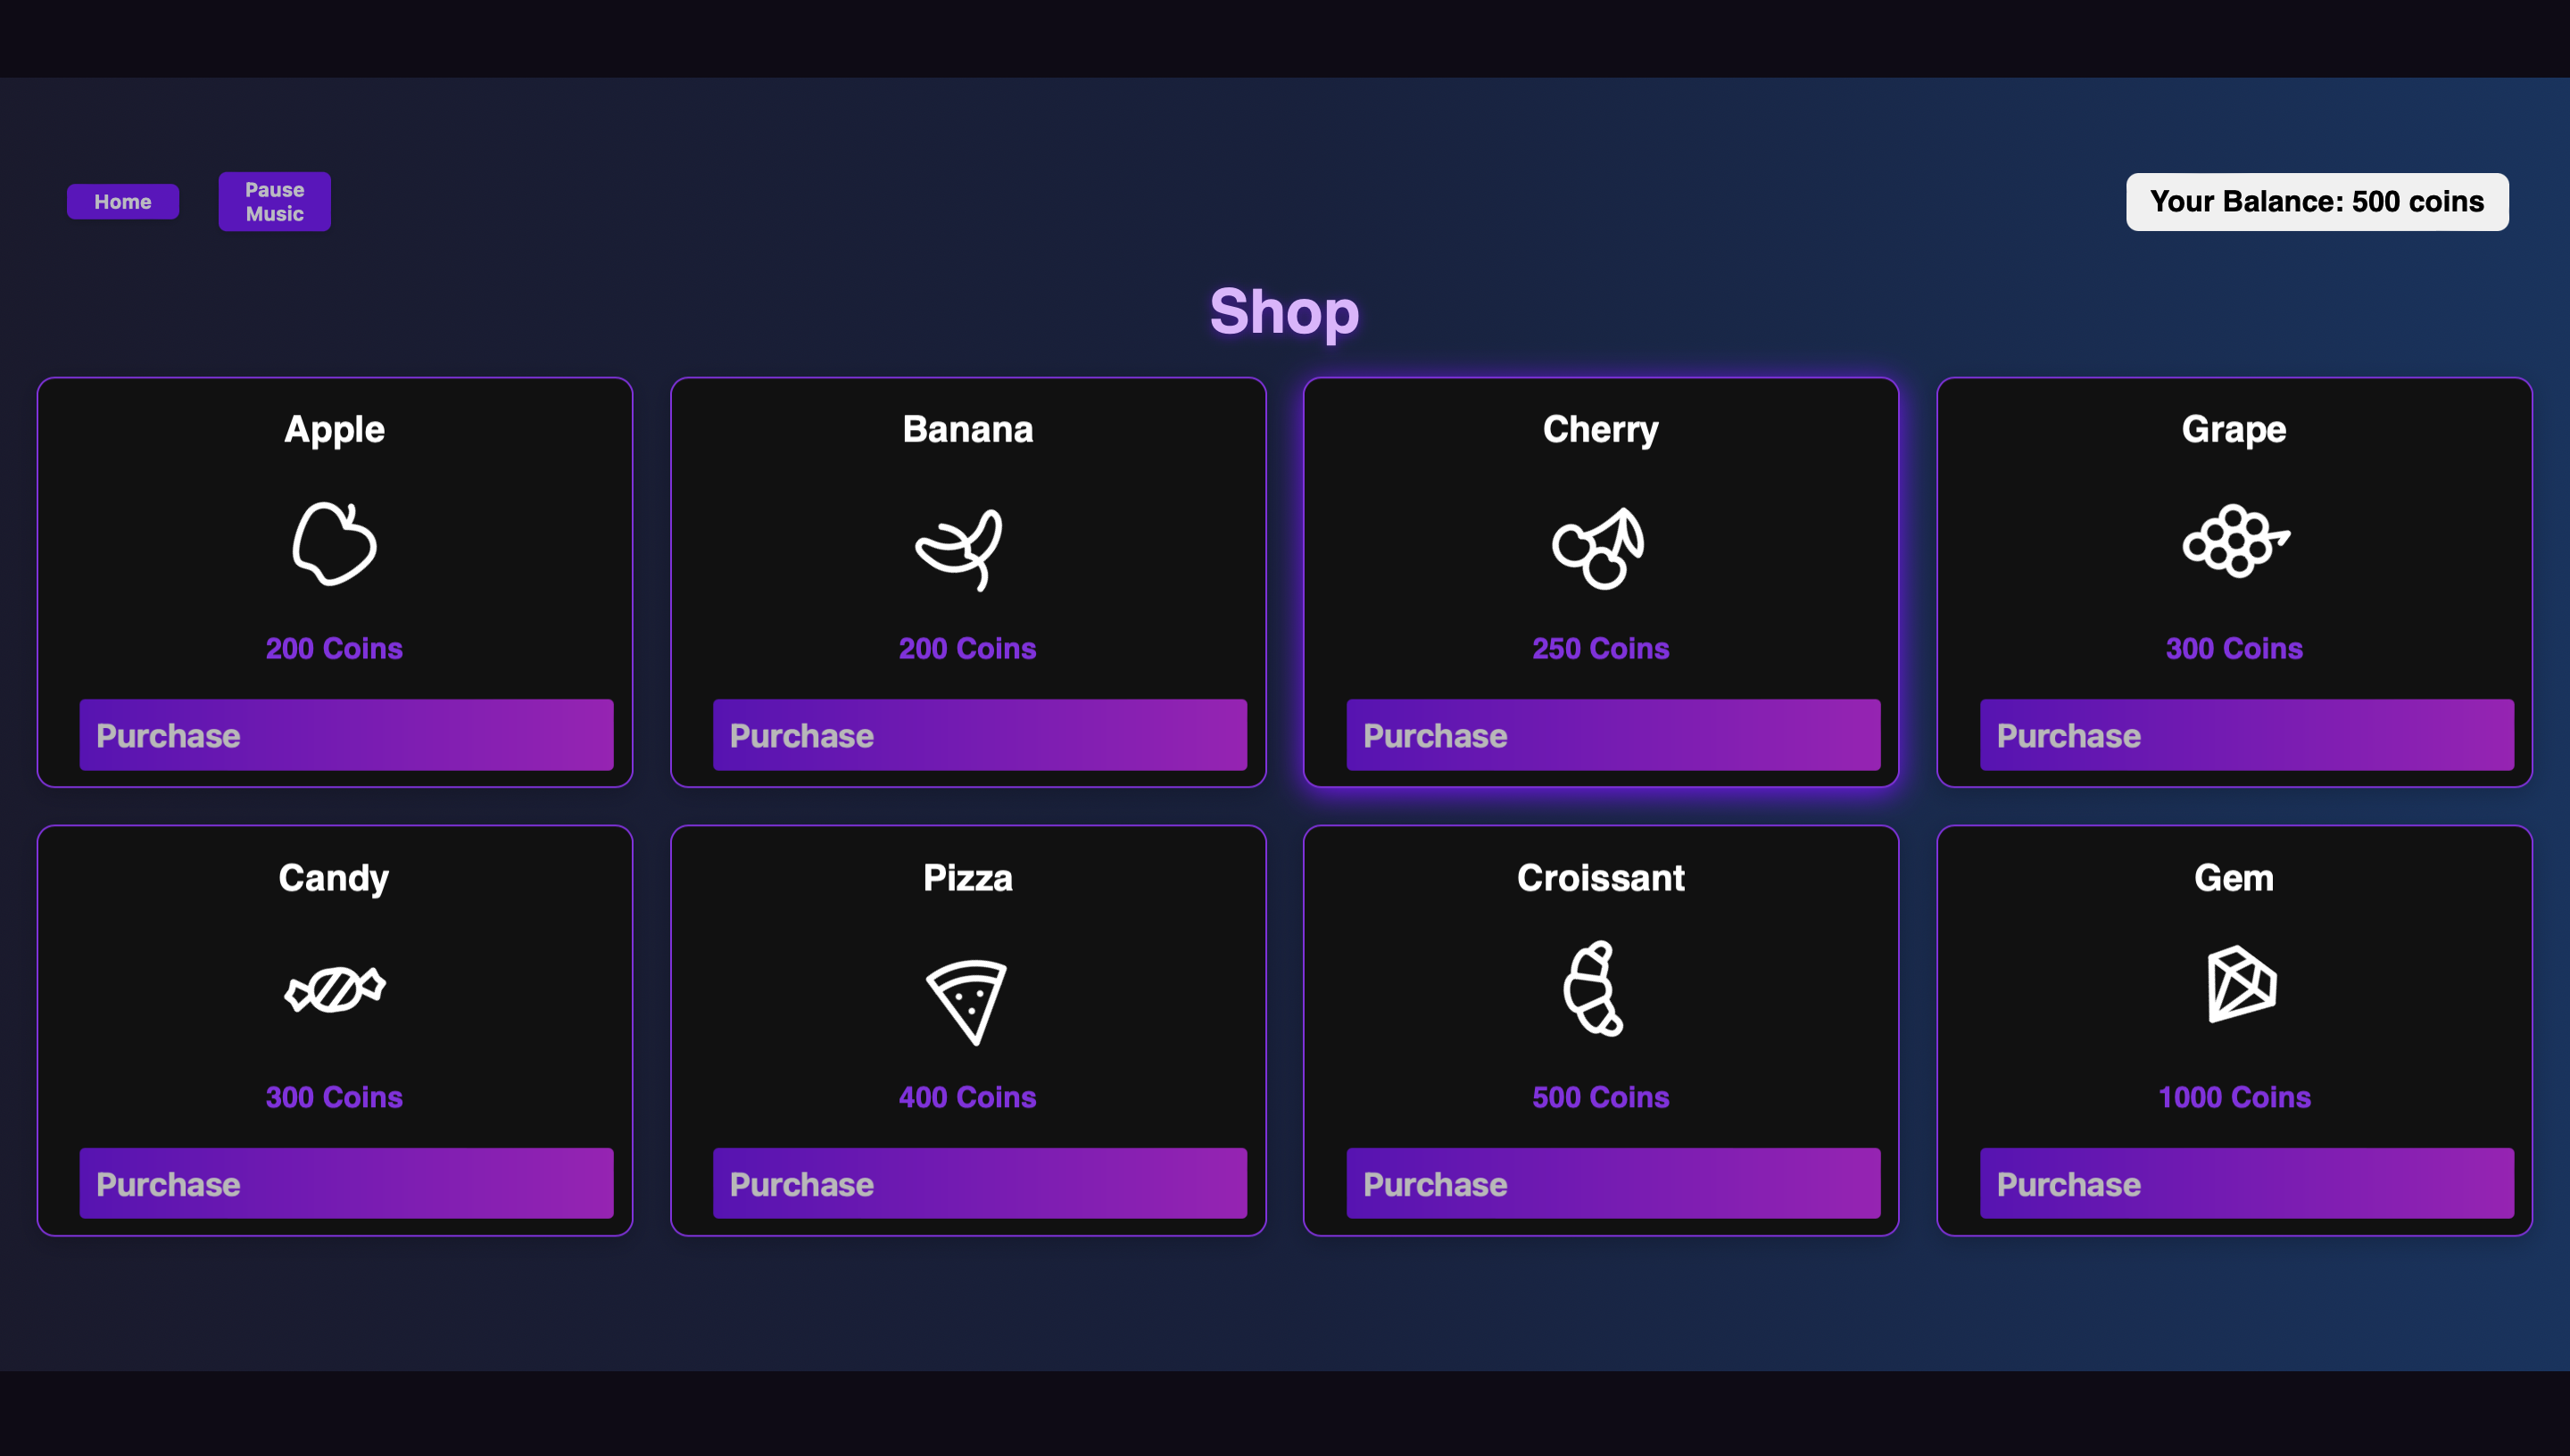
\includegraphics[width=1\linewidth]{UI Screenshot 4.png}
\label{fig:ui4}
\end{figure}

\begin{figure}[h!]
\centering
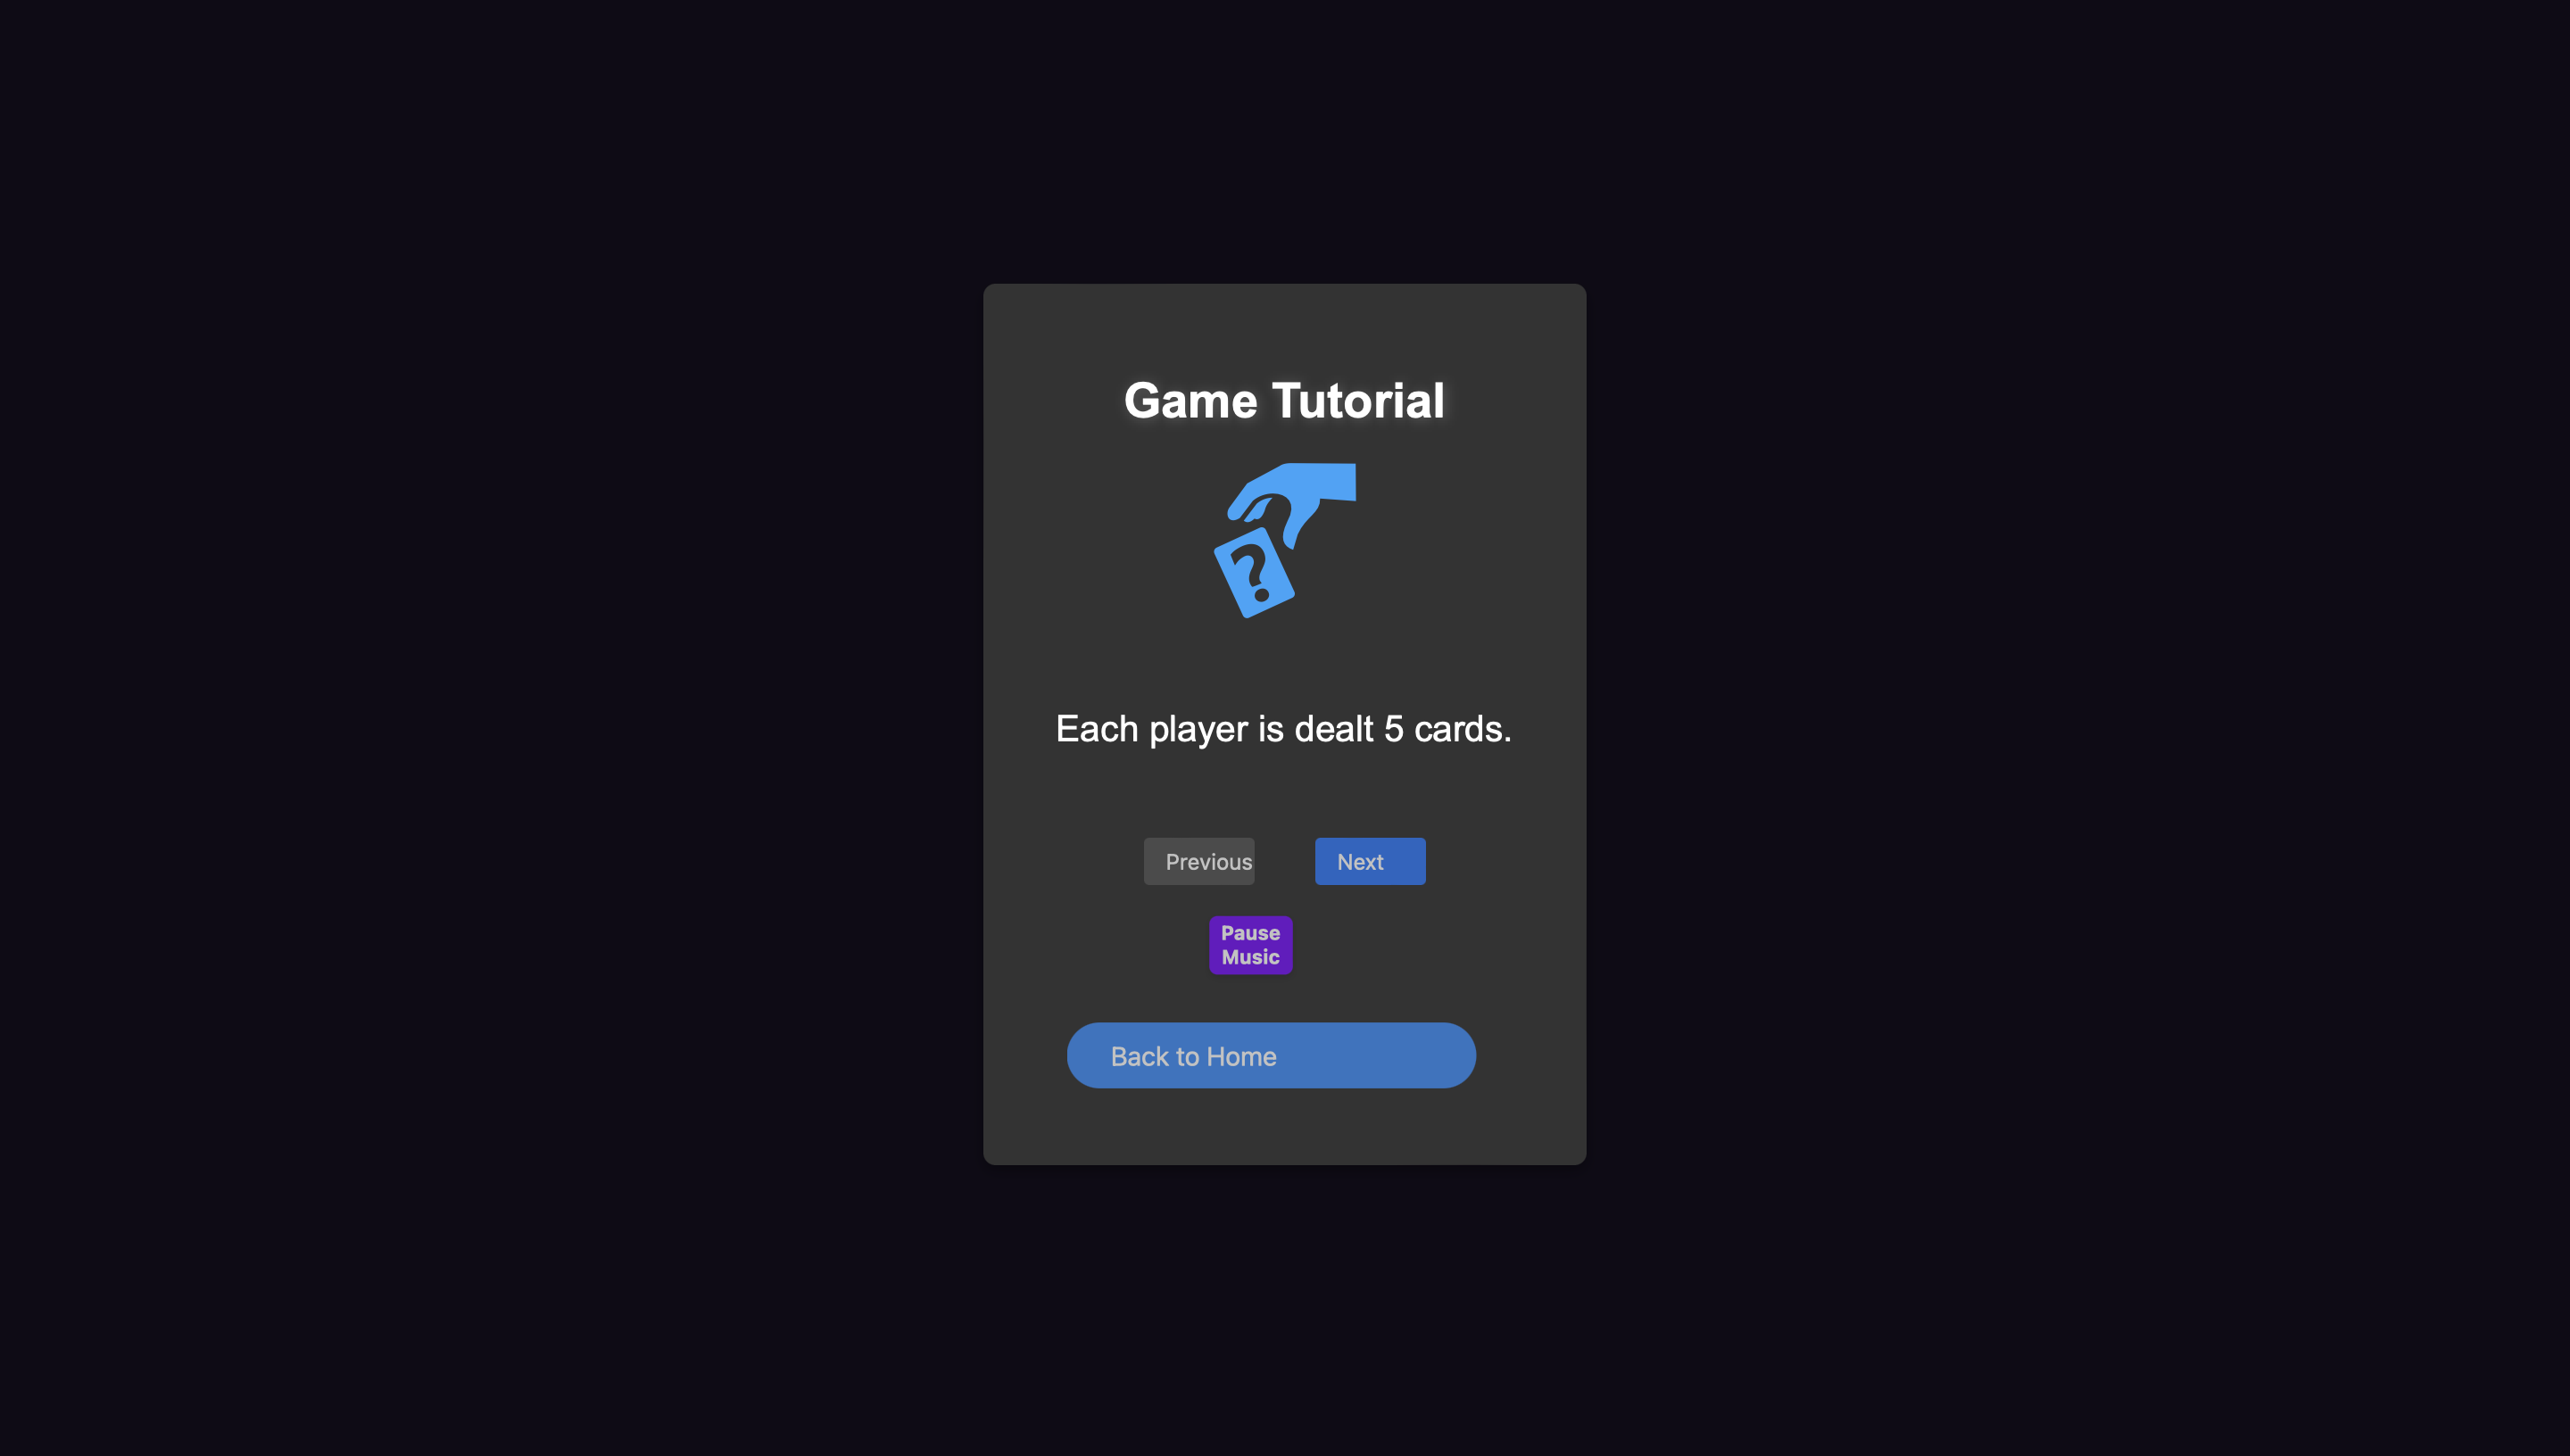
\includegraphics[width=1\linewidth]{UI Screenshot 5.png}
\label{fig:ui5}
\end{figure}

\begin{figure}[h!]
\centering
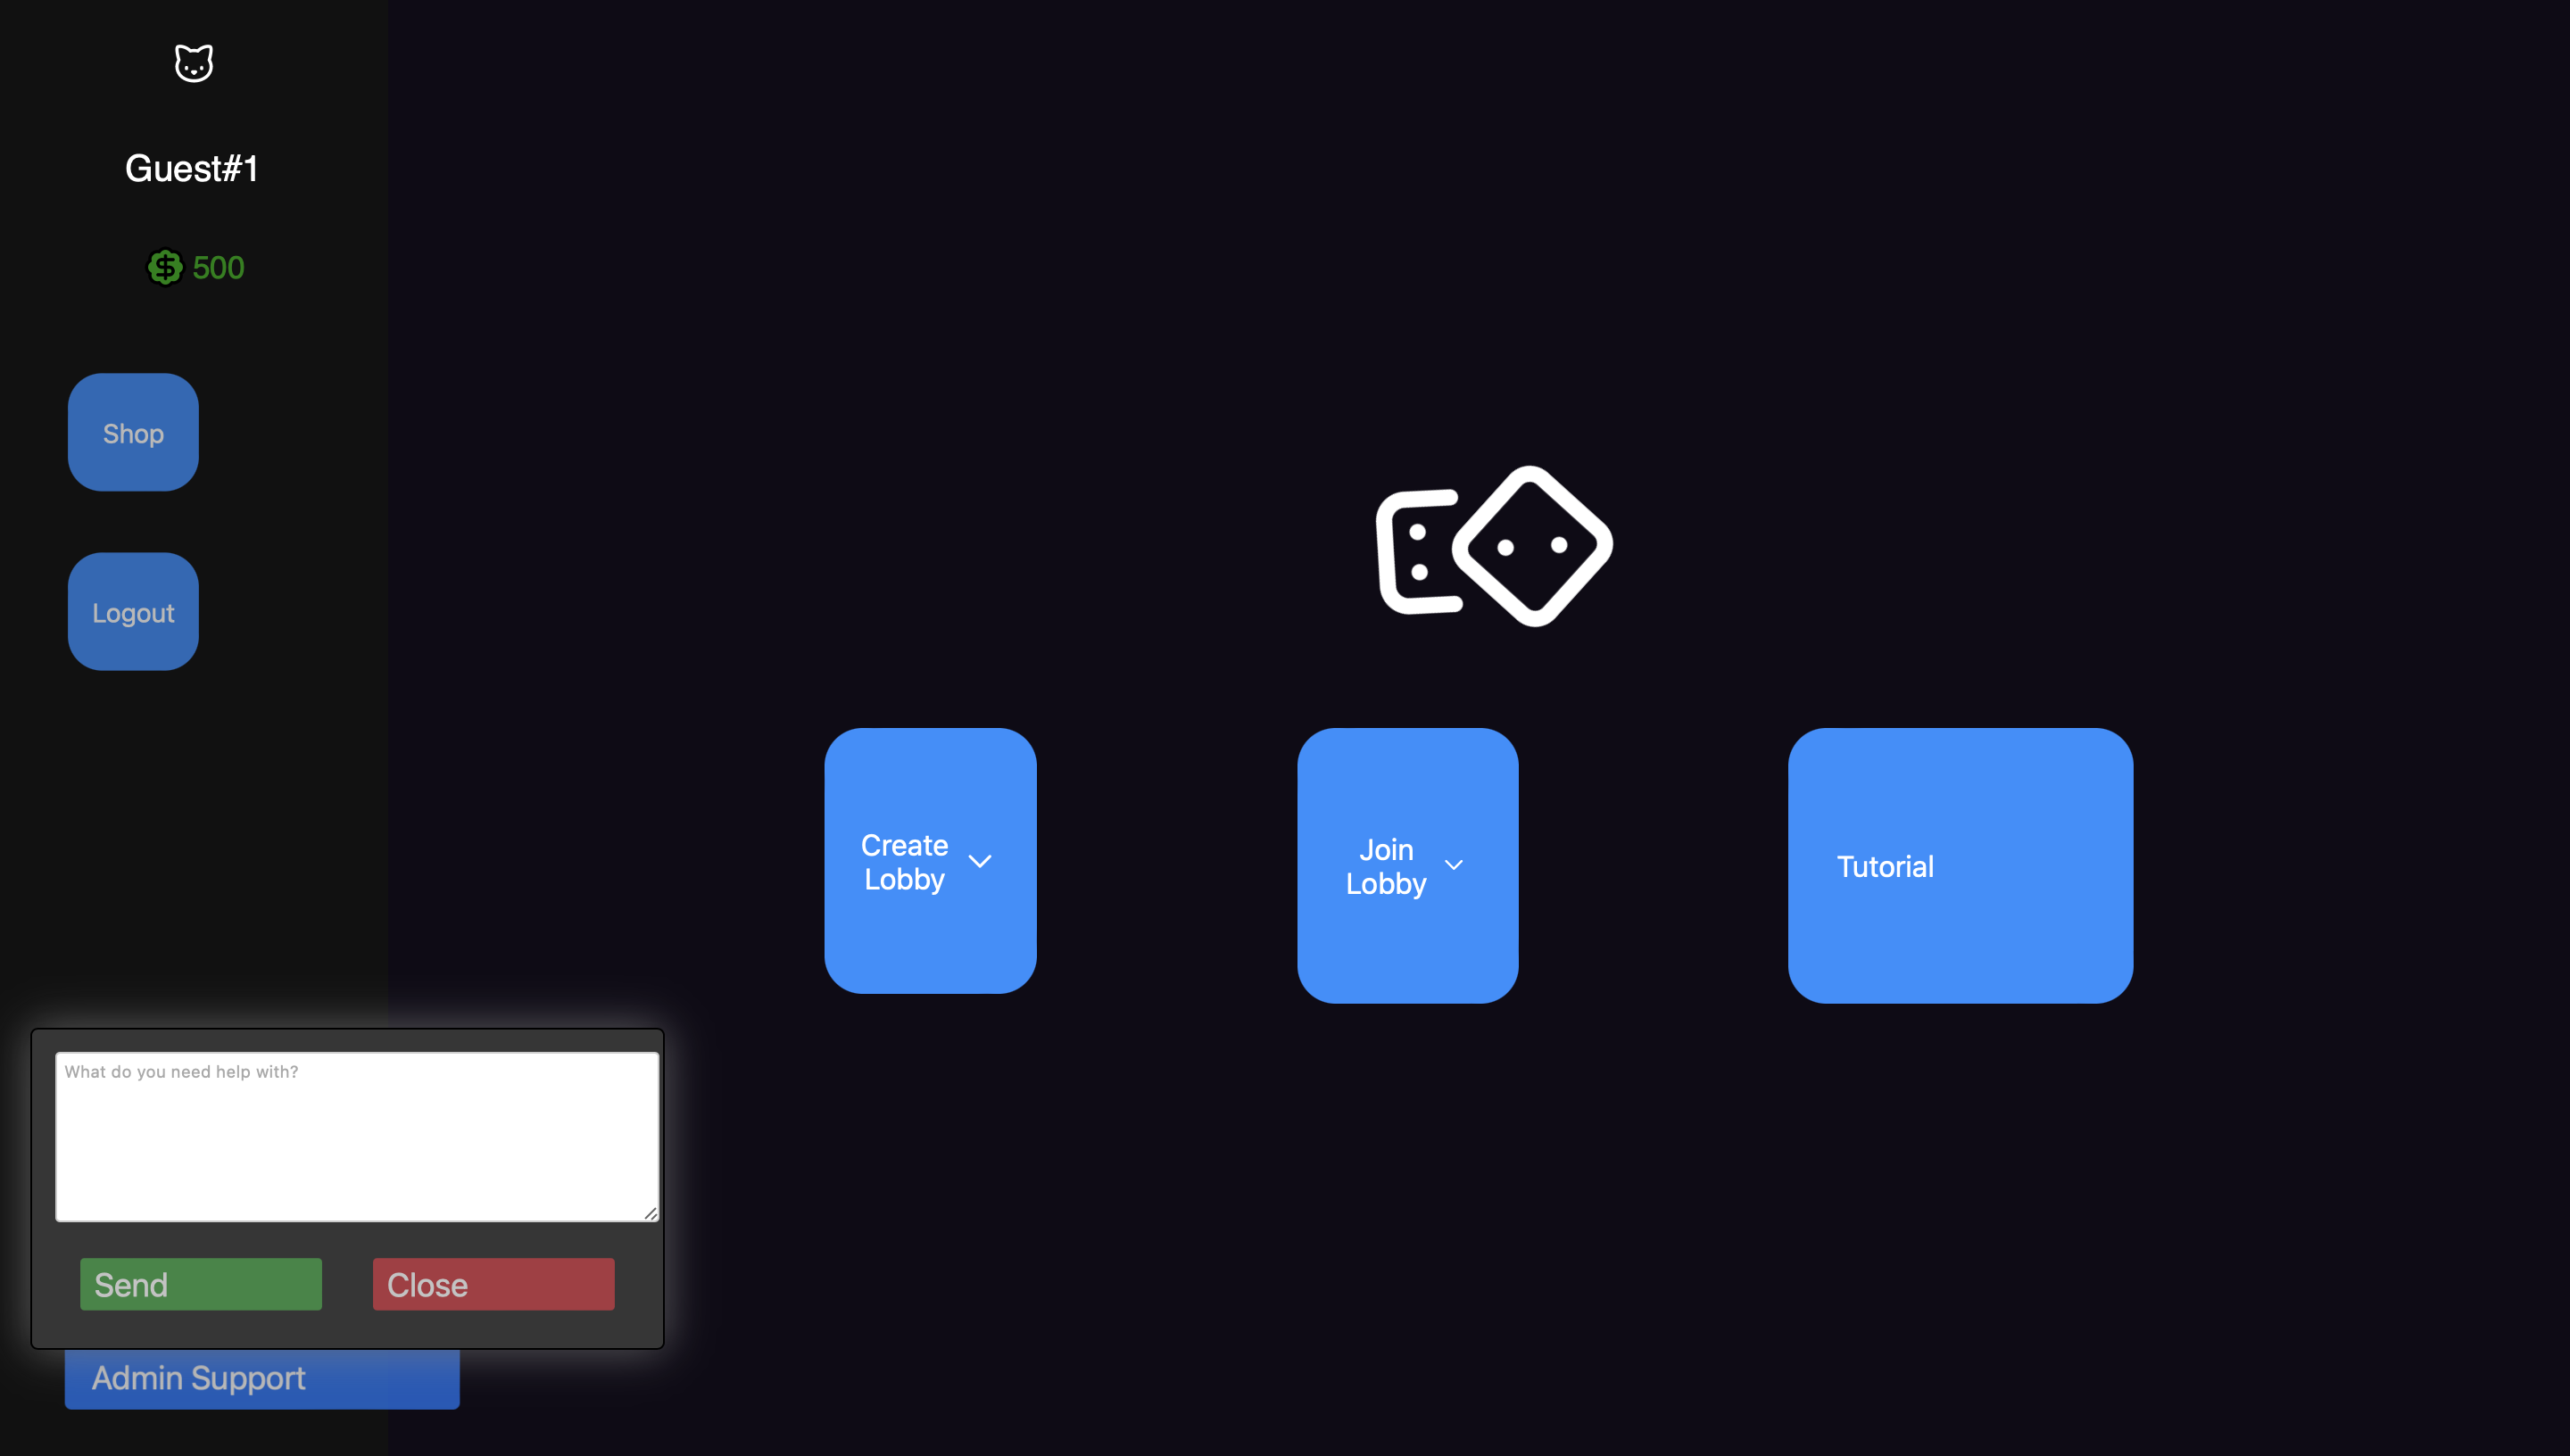
\includegraphics[width=1\linewidth]{UI Screenshot 6.png}
\label{fig:ui6}
\end{figure}

\begin{figure}[h!]
\centering
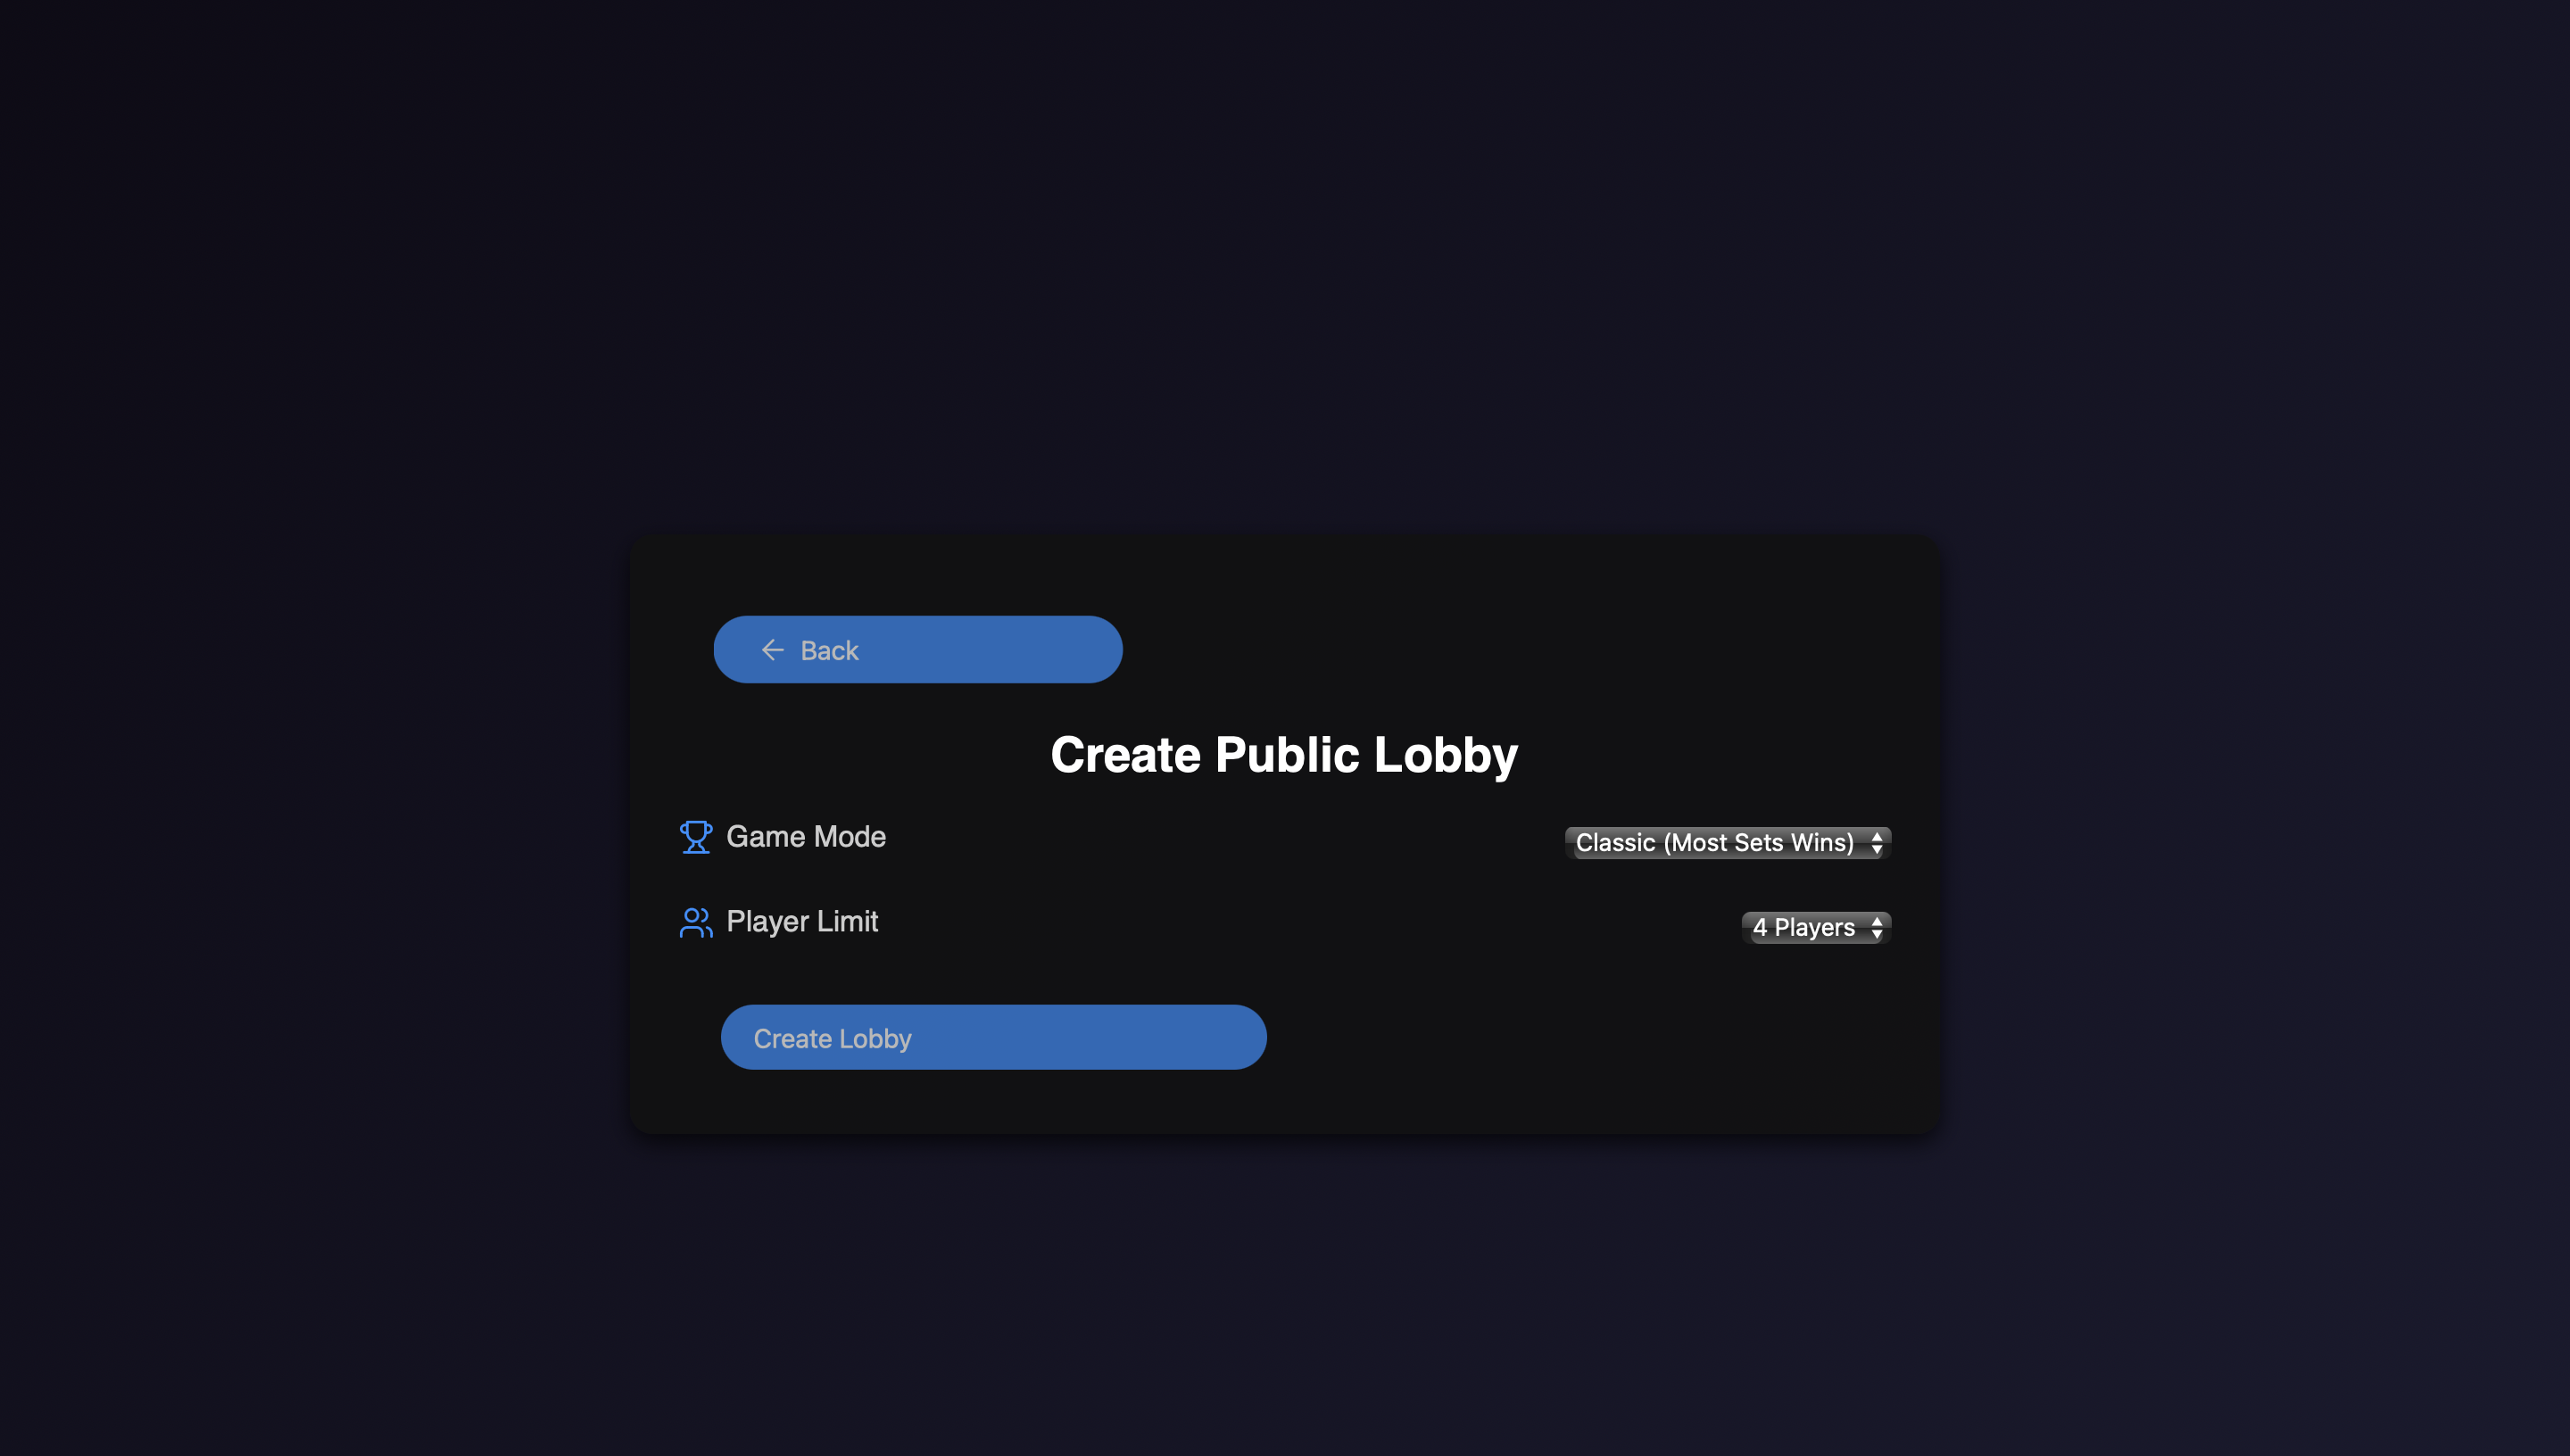
\includegraphics[width=1\linewidth]{UI Screenshot 7.png}
\label{fig:ui7}
\end{figure}

\begin{figure}[h!]
\centering
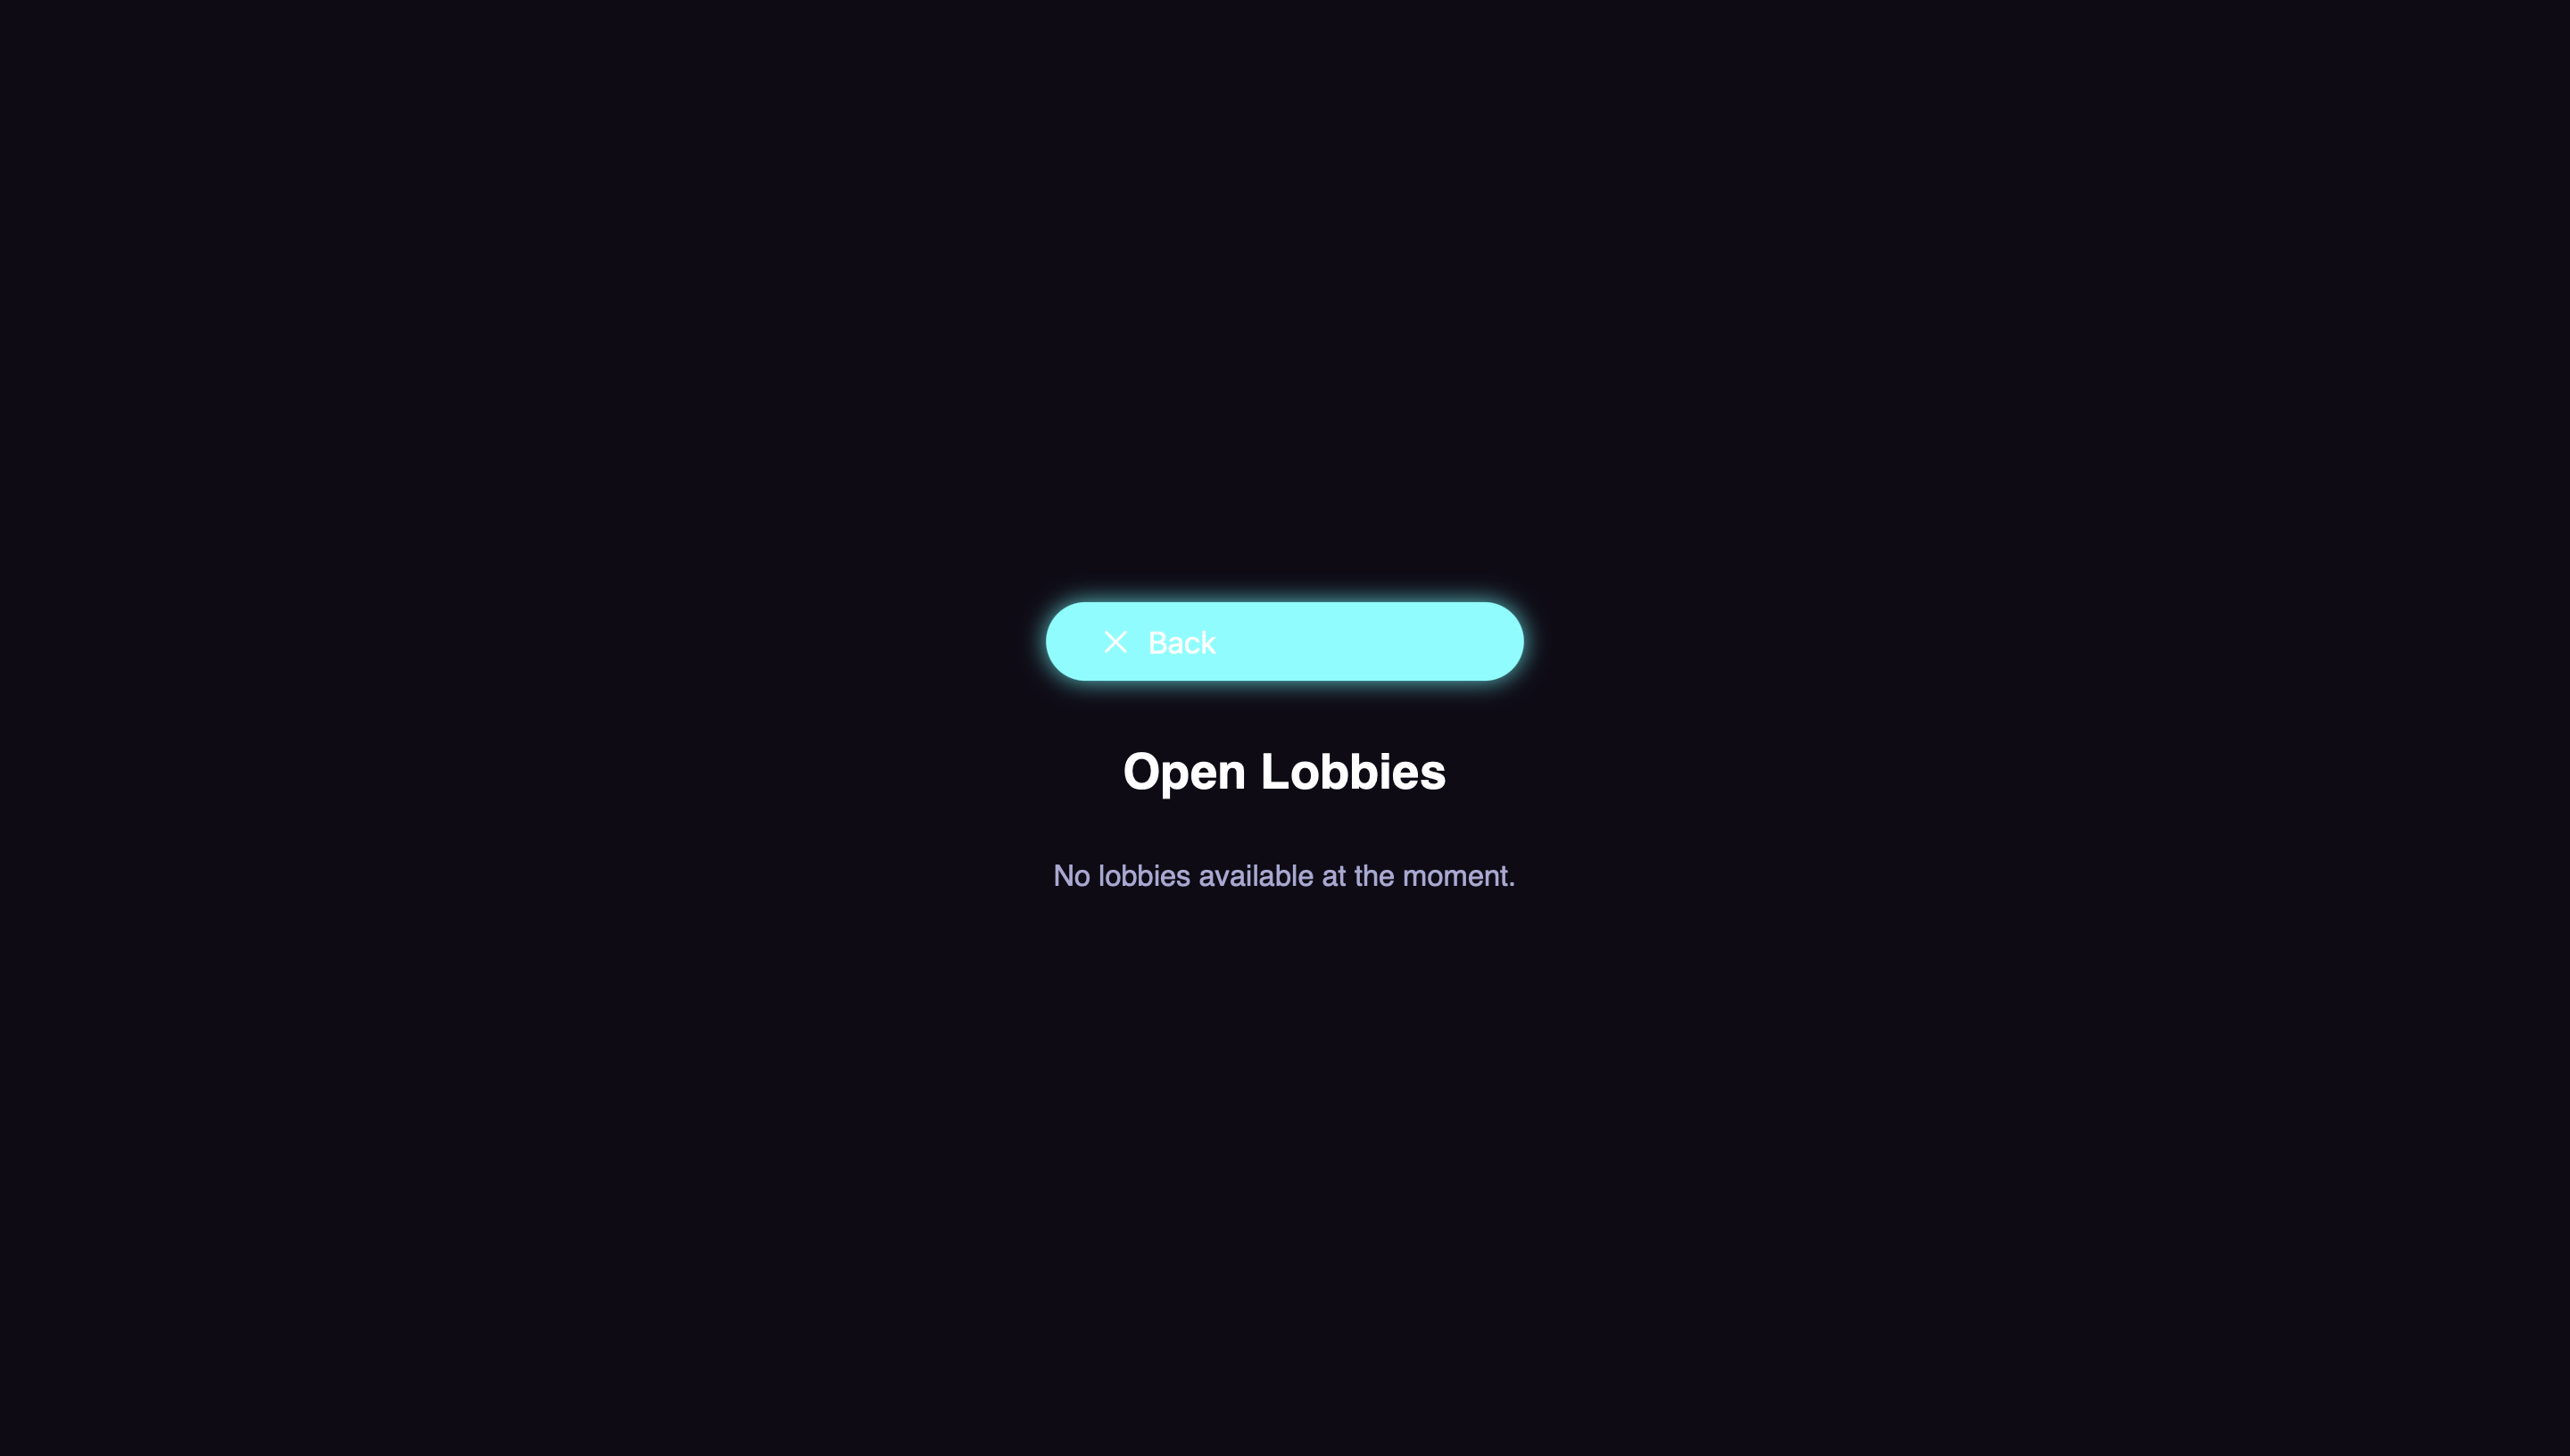
\includegraphics[width=1\linewidth]{UI Screenshot 8.png}
\label{fig:ui8}
\end{figure}

\begin{figure}[h!]
\centering
\includegraphics[width=1\linewidth]{UI Screenshot 9.png}
\label{fig:ui9}
\end{figure}

